\documentclass[12pt, a4paper, oneside]{article}

\usepackage[a4paper]{geometry}
\geometry{verbose,tmargin=1in,bmargin=1in,lmargin=1in,rmargin=1in}

\usepackage{amsmath}
\usepackage{hyperref}
\usepackage{graphicx}
\usepackage{lastpage}
\usepackage{setspace}
\usepackage{fancyhdr}
\setlength{\headheight}{15.2pt}
\pagestyle{fancy}
\lhead{Group: 35}
\chead{Onyx - cloud music library manager\\Design Brief \& Specification}
\rhead{Date Revised:\\ \today}
\cfoot{Page \thepage\ of \pageref{LastPage}}

\newcommand{\env}[2]{\begin{#1}#2\end{#1}}

\begin{document}
\setcounter{page}{0}
\thispagestyle{empty}

\begin{center} \*\\
    \vspace{40mm}
    {\Large The Chinese University of Hong Kong\\Department of Computer Science and Engineering} \\ %School
    \vspace{20mm}
    \hfill \\
    {\Huge Onyx - cloud music library manager} \\ %Heading
    \vspace{8mm}
    {\Large Design Brief \& Specification} \\ %Sub-Heading
    \vspace{20mm} 
\end{center}

\begin{minipage}{0.5\textwidth} %Title page left
    \begin{flushleft} \large

        \emph{Group 35 Members:}\\
        Boris Yau (1155040871)\\
        Fan Wai Keung (1155047303)\\
        FAN Sin Tat (1155047763)\\
        Li Bochao (1155043299)\\
        Tse Cheung Yuet (1155049118)
        \vspace{8mm}

    \end{flushleft}
\end{minipage}
\begin{minipage}{0.4\textwidth} %Title page right
    \begin{flushright} \large

        \emph{Literature Number:} \\
        DS0001a \vspace{8mm}

        \emph{Date Revised:} \\
        \today \vspace{8mm}

    \end{flushright}
\end{minipage}

\newpage
\tableofcontents % Table of Contents

\newpage
\section{Introduction}

\subsection{Project Overview}

Nowadays, there are many website and software related to music streaming.
For example: Spotify, ITunes, Google Music and SoundCloud.
But there are still some groups of people who cannot be satisfied by the existing service,
therefore, we hope to fill out the gap that current music streaming services have left out.\\ 

Introducing “Onyx”. A cloud music streaming and library manager. This platform will provide
several features, such as music access across all platforms via browser,
lossless music playback, large music library handling, cloud music storage and
powerful search engine. The music manager will be separated into public and private music pools
in order to handle copyright issues illustrated by the figure below:

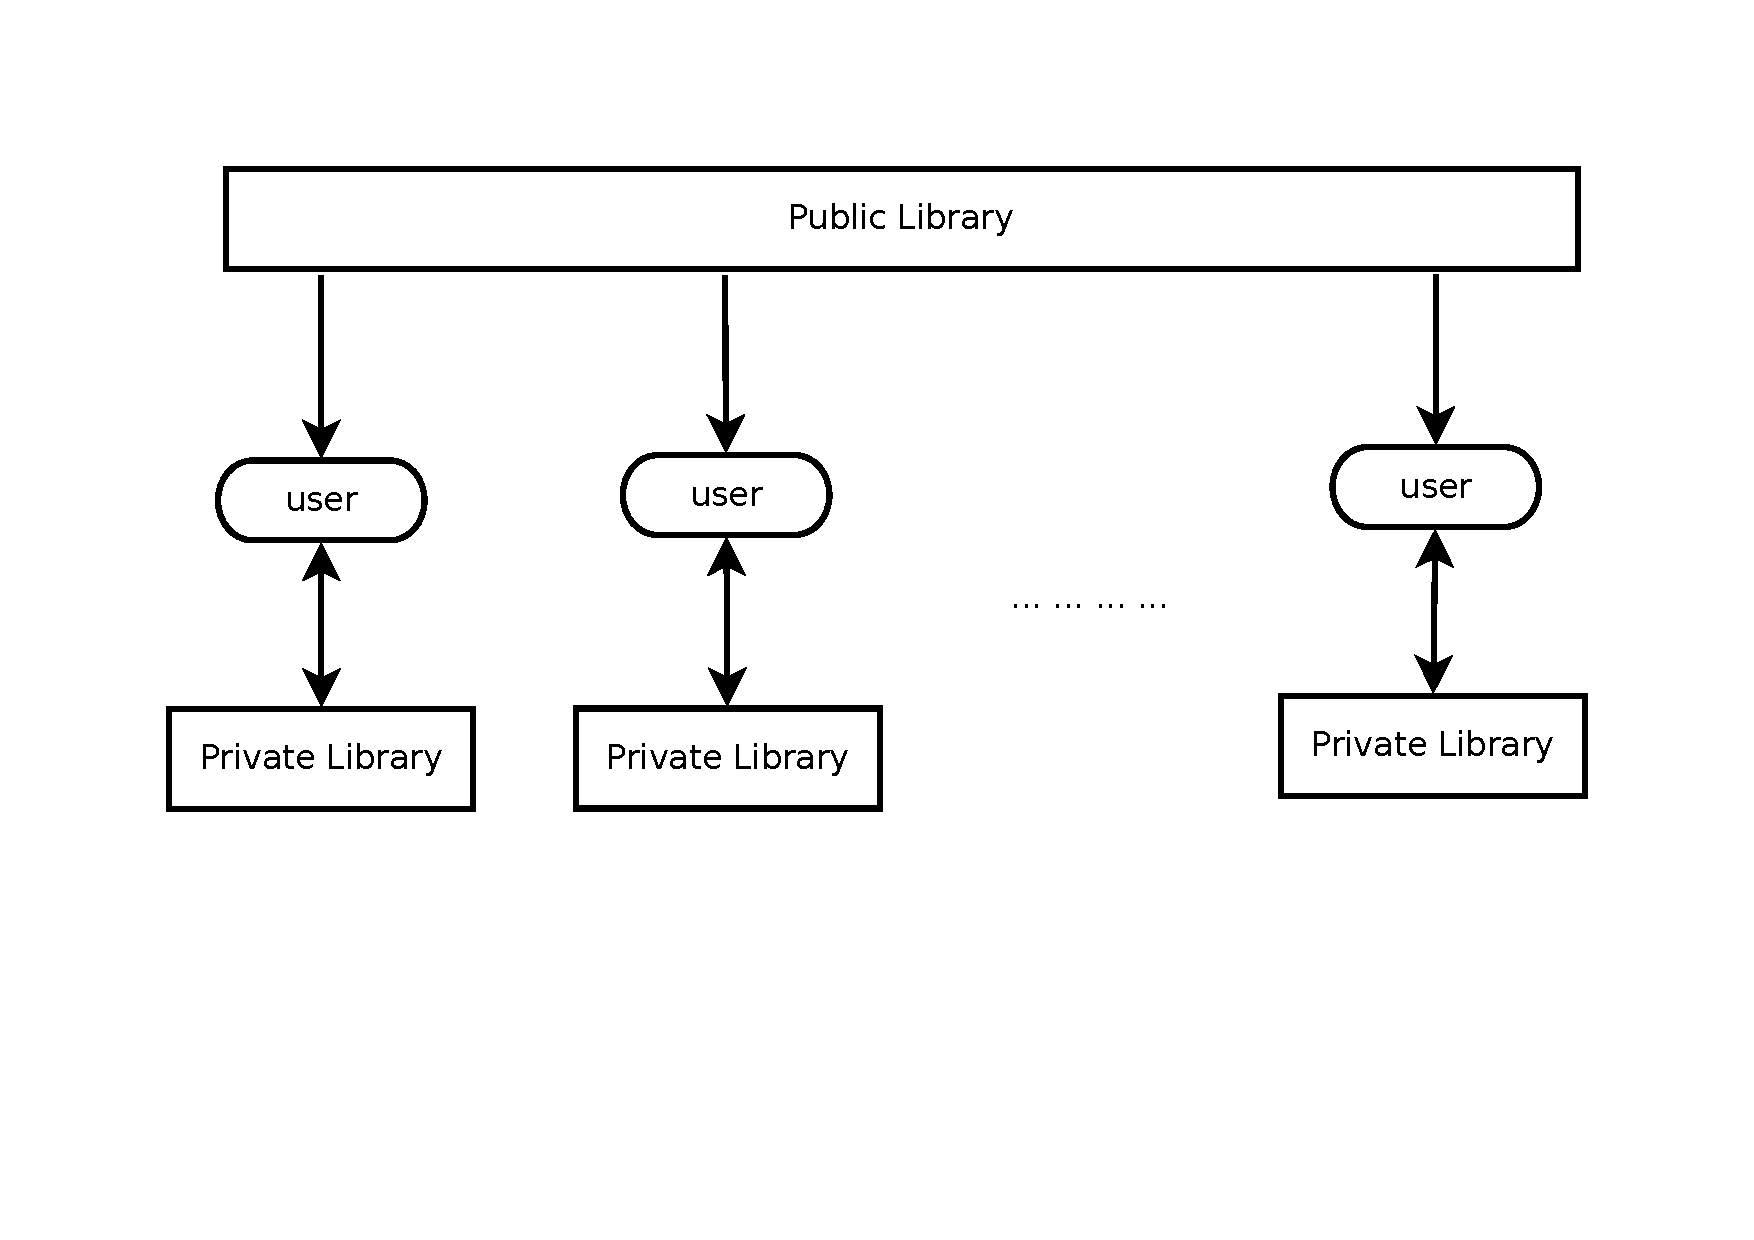
\includegraphics[trim = 25mm 60mm 10mm 20mm, clip, width=\textwidth]{fig/media-access}

For public music pool, we mainly provide copyright-free music, japan anime song and 
other ACG related music, because those music are rare in current music streaming provider.
A subscription fee available for high quality and lossless music playback.\\

As for cloud music storage, we will provide each user with 2GB of music storage for free,
with additional storage available for extra price. One of our feature of cloud music storage is
lossless music playback and download, users can upload their favorites music onto our website
and we can stream the music back to user computer or mobile phone in lossless format and
download back the original file to the user.\\

\newpage
\subsection{Objective}

We hope to provide indie music and Japanese anime music on our platform.
Music is an important culture in the world. However, these kinds of music are not available
on most of the music streaming platform in Hong Kong. It is a headache for music lovers
who prefer to listen to these unpopular songs. Our platform would be a solution for them,
due to the genres of music that our public music pool would provide.\\

Apart from this, we also aim to develop a music platform that allows users to enjoy high quality
music across different computers. We believe that a song is not only a part of the
popular culture, but also a piece of art. By using our lossless music streaming service,
music lovers could enjoy beautiful music and listen to the details of songs easily.\\

We hope that our platform would be user-friendly and easy-to-use. User experience is an essential
quality that we will consider during the development. If the user interface and the flow of
managing music are not user-friendly, the users may not want to use it again. Therefore,
we decided to provide a music manager with clean and intuitive design.\\

\subsection{Expected Customer and Market}

Our platform is designed to target at two types of users -- (1) audiophiles;
and (2) indie music and Japanese music lovers. The two main functions of the platform are
closely related to these two groups of stakeholders.\\

Firstly, our lossless music streaming service is suitable for audiophiles,
people who enjoy listening to high quality music. Although there are existing online music
library service, such as Google Play Music, they always compress the music on their server
before streaming to save bandwidth. Therefore, their services may not fulfil the audiophile's
needs. In contrast, our platform may fit their preferences in listening to high quality music.\\

Besides, our platform also aims to provide services for indie music lovers and Japanese anime
music lovers in Hong Kong. There are several music streaming providers in Hong Kong, such as
Spotify, MOOV, KKBOX and JOOX. All of them offer a vast music database to users. However,
music tracks on these platforms are usually popular. Indie music lovers and Japanese anime music
lovers cannot listen to their favourite music on these existing platforms. There are many
kind-hearted music players who are willing to share music to the public domain or by Creative
Commons license. We will be able to add their music to our public pool legally.
This is a win-win situation that the music lovers could enjoy these music and the music players
could promote their music to the public.\\

\newpage
\subsection{System Features}

\noindent Search Engines: \env{itemize} {
\item Simple search: search by keyword of song, album and Artists.
\item Advanced search: can filter to specific album and artists to find keyword of song.
}

\noindent Upload music and playlist: \env{itemize} {
\item Free 2GB of storage is given to user 
\item User can upload their own lossless music to the system and create custom playlist mixed
    with public music pool and cloud music pool
\item User can name their custom playlist
\item User can store the whole album in public library as his/her own playlist
}

\noindent Streaming and download: \env{itemize} {
\item User can choose playback as lossless format to obtain the maximum music quality
    or normal mp3 formal to save mobile data usage for mobile user  
\item User can download their own music back to their computer and remain untouched,
    also some of the copyright-free music in our public music pool can also be downloaded.
}

\noindent Playback: \env{itemize} {
\item Different playback mode will be provided, include sequential,
    single song loop, album or playlist loop and random.
}

\noindent Tag: \env{itemize} {
\item User can edit their cloud library song tag, make it easier to manage if library is large.
\item Support multi-song tagging at same time, auto tagging based on online resources may be provided.
}

\noindent Now playing: \env{itemize} {
\item Current playing play list will be display to let user to quickly change the song.
}

\noindent Administrative Features: \env{itemize} {
\item Extra page will appear then login in as admin, this administrator page enable admin to
    manage public music pool, for example, add, edit and delete operation,
    this also include user account management.
\item Real time server loading can be monitor, include CPU, HDD loading and RAM usage.
}

\newpage
\section{Background}
Online music streaming services have become more and more popular due to the rise of Spotify,
Google Music and Apple Music. Among these three music streaming services, only Google provides
cloud music storage for users. However, users can only store no more than 50000 songs, and the
songs will be compressed to 320 kbps mp3, no matter what quality the user uploads. We aim at
dealing with this weakness of current music streaming providers, which are unable to provide users
with lossless music playback and storage. We shall allow users to upload lossless music to our
servers, and stream them at anytime and anywhere they want. Our server will not compress the
uploaded music, and will maintain their original quality during playback.\\

As for the current music streaming services, a lot of the songs are region restricted.
For example, you cannot listen to some Japanese pop/anime songs if you are not in Japan.
We aim to lift this restriction, and try to provide global license for all our public music
streaming. We want all our customer to enjoy music as they were supposed to, and not worrying
about some songs unable to be streamed in certain regions.\\

As for music genres, most music streaming services only focus on popular pop music such as
Taylor Swift, Eminem for the US, Eason Chan, Jay Chou etc for the Chinese market. Almost all
of the music providers lack anime and indie music. From our knowledge, Spotify basically only
has a tiny portion of songs which is in Japanese, as for Google Music and Apple Music, most
Japanese music are restricted to be streamed (and bought) in Japan only. We aim to solve this
problem by only focusing on a small portion of the music (mainly anime and indie music), the gap
where most main music streaming companies does not provide. By only providing anime and indie
music, we can spend extra money to buy global copyright license of the music.\\

Our music manager will contain both music subscription feature, as well as music storage feature.
Both of these payment method will work, and the reasons are as follows. 

\env{enumerate} {
\item For audiophiles, they have already paid thousands of dollars for great headphones,
    Hi-Fi players and amps, thus they are definitely willing to pay a small sum of monthly
    subscription fee in order to listen to lossless music, which are hard to find elsewhere.
    As for online music storage, if they have a large music library, paying to keep their music
    as a backup in original quality, as well as able to stream them anywhere at anytime is a
    very attracting offer.
\item For anime/indie song lovers, it’s very hard to find copyrighted songs which can be
    streamed online. They either have to illegally download them, or buy those expensive
    imported CDs from Japan and rip the music themselves. If there is a platform which provide
    anime music streaming, I think a lot of people will be willing to pay instead of spending
    time finding illegal BT seeds or buying expensive CDs. 
}

Overall, we think that there is definitely a market place for our music manager, and we believe
we can provide a comfortable and legal music playing environment for our customers.

\newpage
\section{System Architecture}

\subsection{Server-Side}
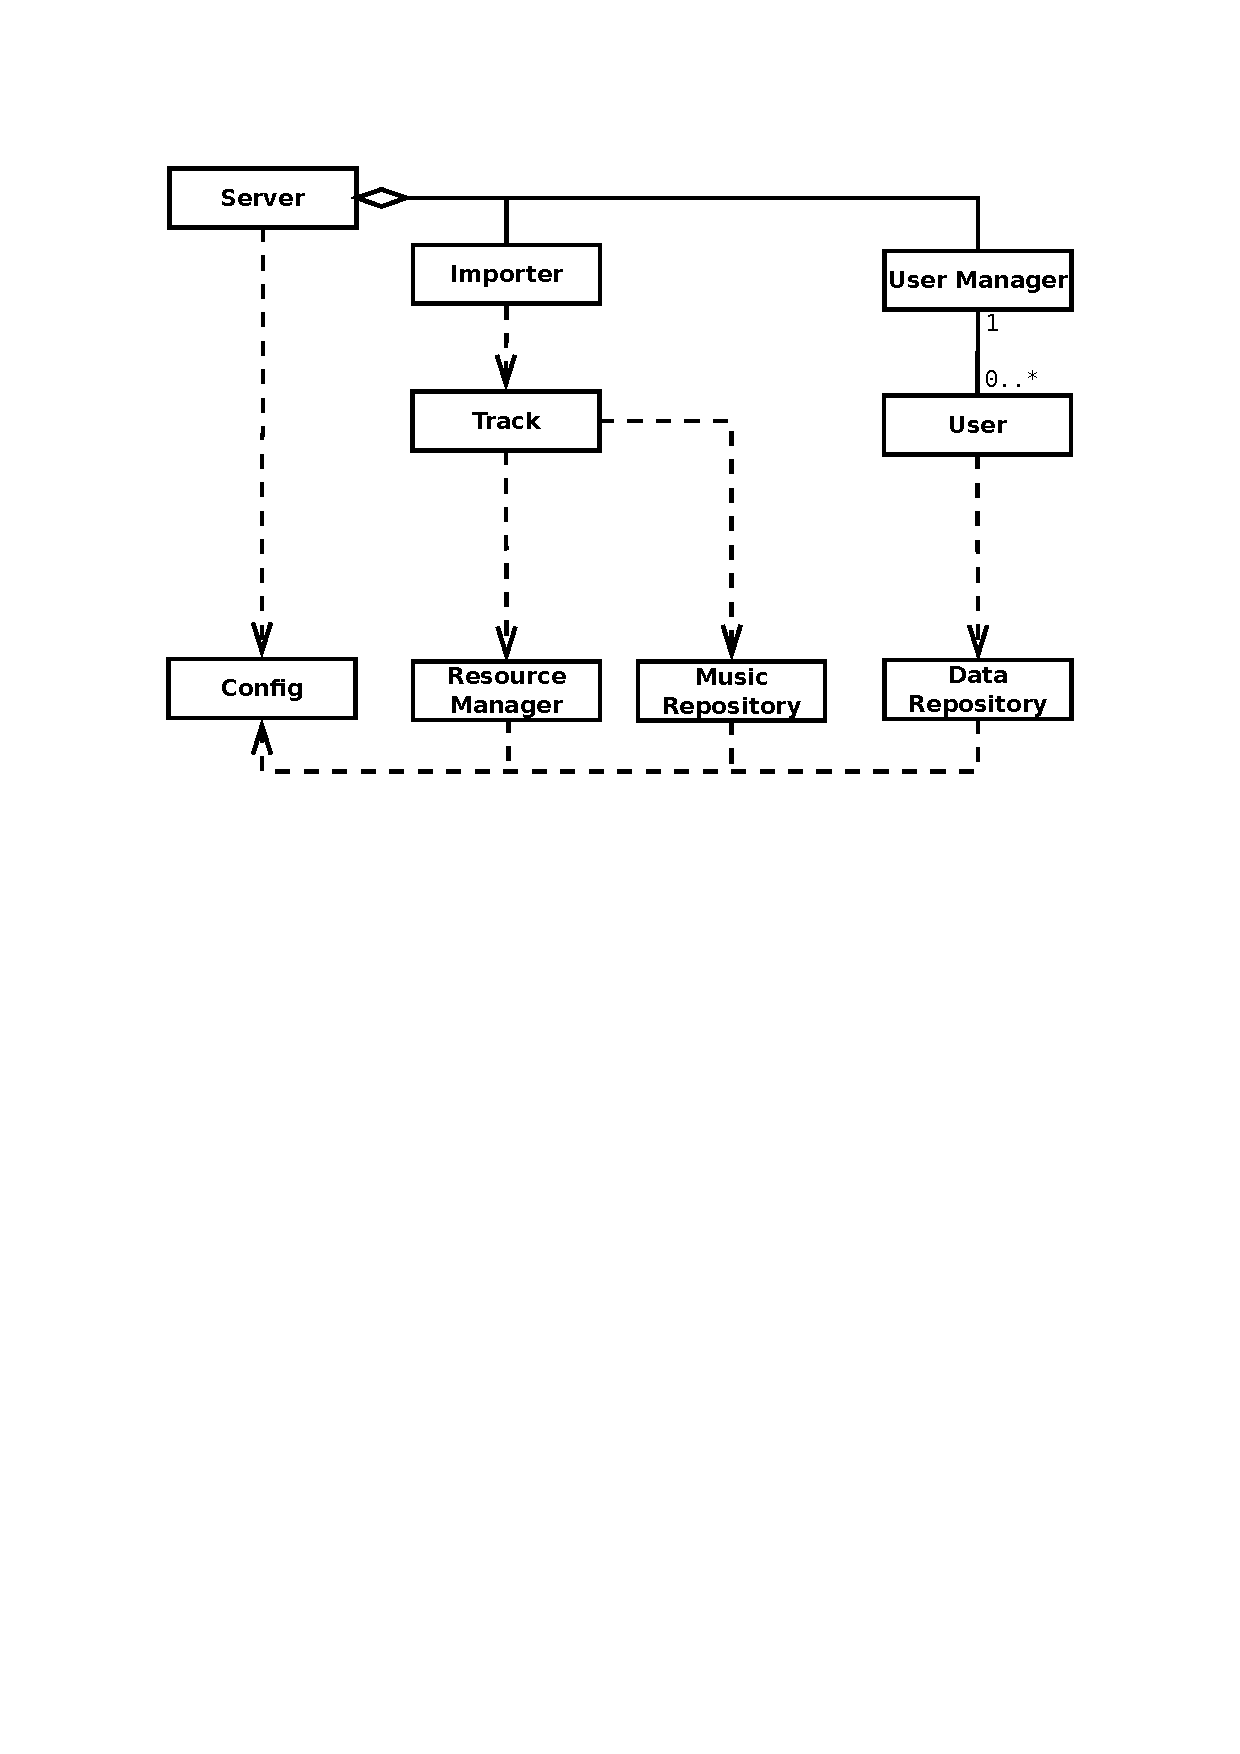
\includegraphics[trim = 25mm 160mm 25mm 20mm, clip, width=\textwidth]{fig/uml_class_Server}
\env{itemize} {
\item Server: Main place for storing user information and music information
\item Importer: The temporary place of uploaded song storage during batch upload
\item Track: Extract the importer data of uploaded song one by one and make record in different database. 
\item User Manager: Manage all the users accounts and authentication system of user
\item User: The user account information(e.g. login names, password)
\item Config: the setting file of Resource Manager, Music Repository, Data Repository and Server
\item Resource Manager: save and manage the music file (e.g. wav, flac, mp3).Also, convert those file into different music format
\item Music Repository: containing the information of each music file (e.g.the singer, album ,tags)
\item Data Repository: containing the information of user (e.g. PlayList, upload history)
}

\newpage
\subsection{Client-Side}
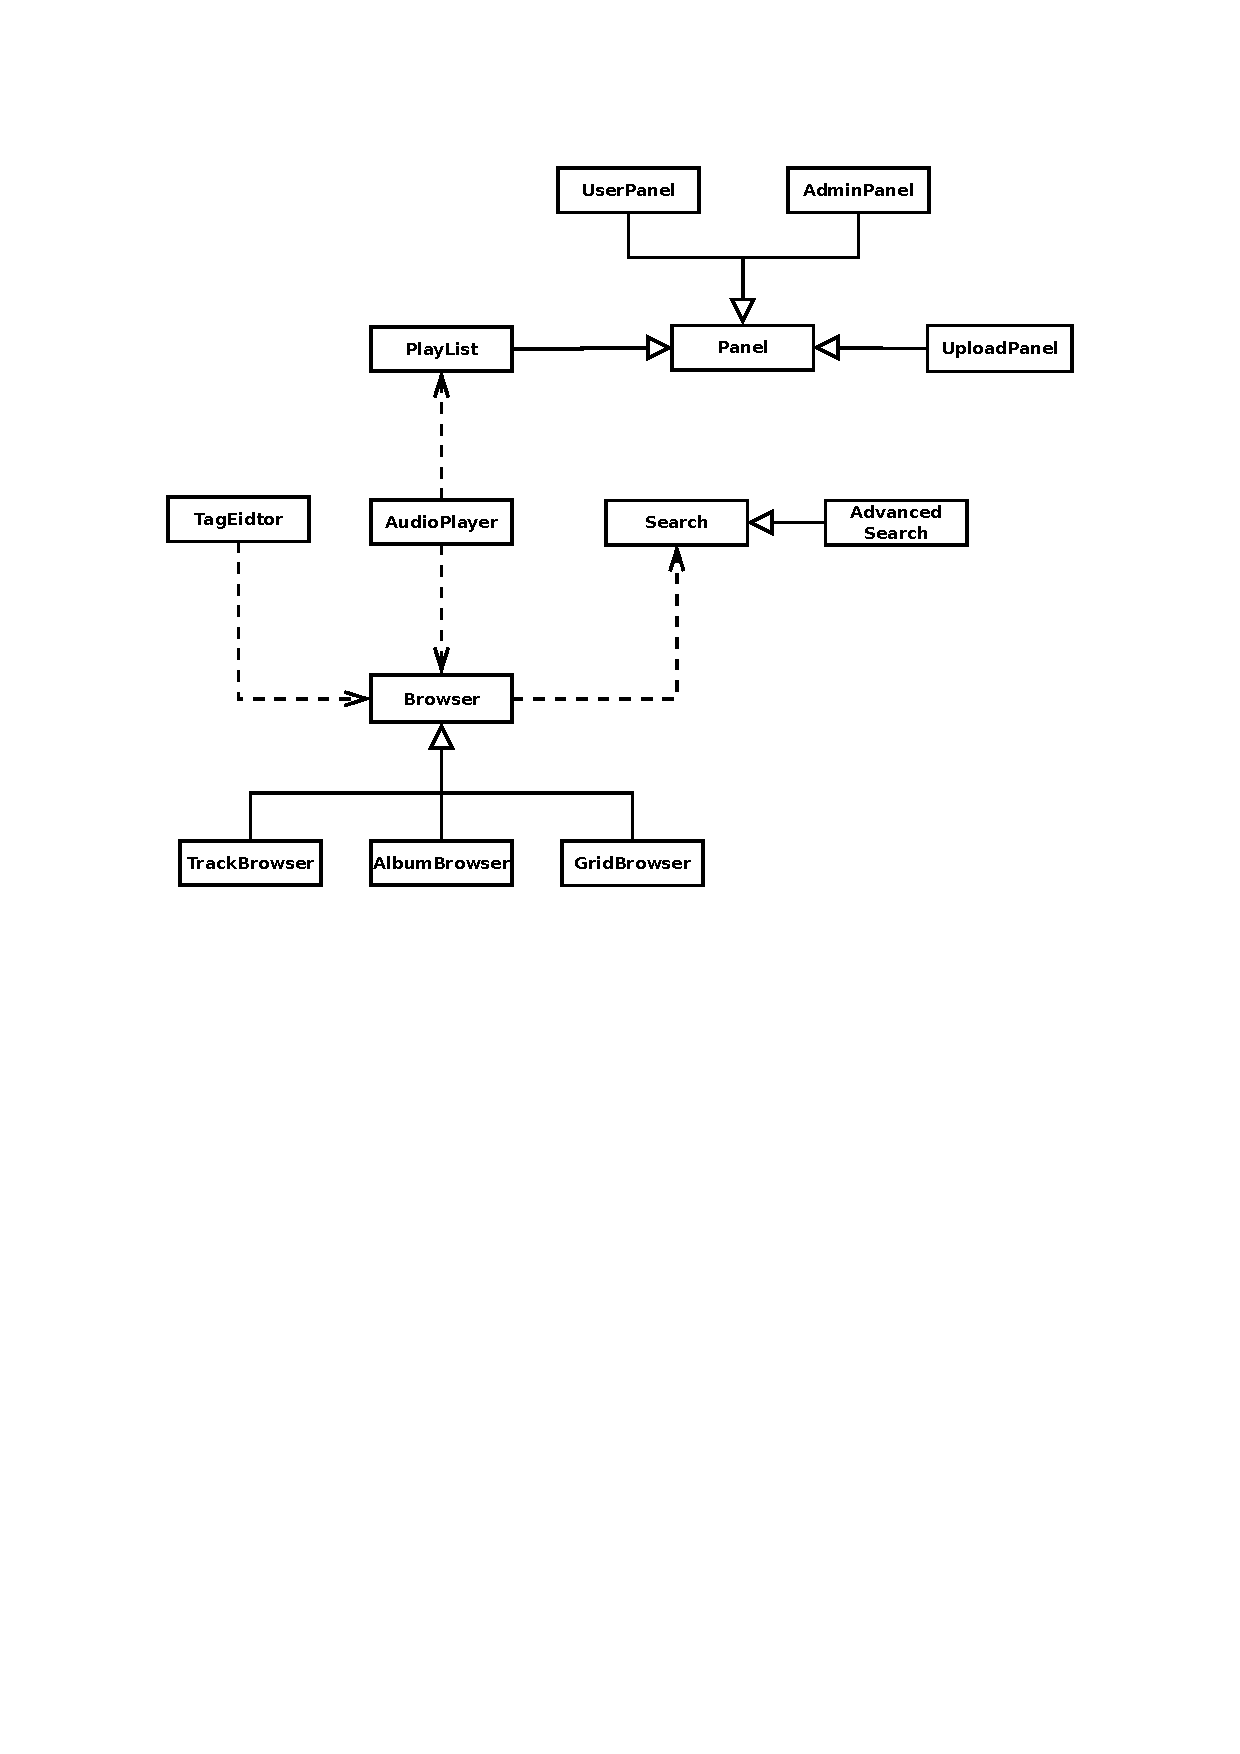
\includegraphics[trim = 25mm 140mm 25mm 20mm, clip, width=\textwidth]{fig/uml_class_Client}
\env{itemize}{
\item Panel: Containing User Panel, Admin Panel, Upload Planel and Playlist
\item User Panel: User main interface, include download, setting page, information of user, etc……
\item Admin Panel: administrating the server library and server states
\item Upload Panel: upload music from user computer
\item Playlist: The list of current playing music
\item Audio Player: control and display the status of music
\item Tag Editor: edit the tag of music
\item Search: searching music by keyword and contain advanced search
\item Advanced Search: Search music by given information and filter option, such as tag, album and singer
\item Browser: Display and browse the music,album or search results. Containing 3 types of browsers
\item Track Browser: Display the detail information of the whole play list, include custom playlist and album list.
\item Album Browser: Display the detail information of Album song list and other information
\item Grid Browser: Display the of picture and rough information of albums or music in grid.
}

\end{document}
